\documentclass[aspectratio=169]{beamer}
\PassOptionsToPackage{english}{babel}
\usepackage{standardslides}

\title{Numerical Relativity: \\ Simulating the Evolution of Binary Black Holes}
\author{Markus Pawellek}

\AtBeginSubsection[]{
  \begin{frame}
    \vfill
    \centering
    \begin{beamercolorbox}[sep=8pt,center,shadow=true,rounded=true]{title}
      \usebeamerfont{title}\insertsubsectionhead\par%
    \end{beamercolorbox}
    \vfill
  \end{frame}
}

\begin{document}
  \frame{\titlepage}
  \begin{frame}{Outline}
    \footnotesize
    \hfill\parbox[t][7cm][l]{0.9\textwidth}{\tableofcontents}
  \end{frame}

  \section{Introduction} % (fold)
  \label{sec:introduction}
    \begin{frame}{Introduction}
      Example:
      \begin{itemize}
        \item{
          \href{run:videos/sxs-bbh-gravitational_lensing_of_gw150914.webm}{\beamergotobutton{SXS: Gravitational Lensing of GW150914}}
          \href{https://en.wikipedia.org/wiki/File:BBH_gravitational_lensing_of_gw150914.webm}{\beamergotobutton{Web Version}}
        }
      \end{itemize}
      \bigskip

      \pause
      What is Numerical Relativity?
      \begin{itemize}
        \item science about numerical solutions to the Einstein field equations
      \end{itemize}
      \bigskip

      \pause
      Why?
      \begin{itemize}
        % \item recreation of cataclysmic cosmic phenomena that are otherwise inaccessible
        \item prediction and explanation of cosmic phenomena and relativistic instabilities
      \end{itemize}
    \end{frame}
  % section introduction (end)

  \section{Background} % (fold)
  \label{sec:background}
    \begin{frame}{Einstein Field Equations}
      \begin{mybox}
        \[
          R_{μν} - \frac{1}{2}Rg_{μν} = \frac{8\pi G}{c^4}T_{μν}
        \]
      \end{mybox}
    \end{frame}
    \begin{frame}{Vacuum Field Equations}
      \begin{mybox}
        \[
          R_{μν} = 0
        \]
      \end{mybox}
    \end{frame}

    \begin{frame}{Analytical Solutions}
      Schwarzschild Metric:
      \[
        (g_{μν})(t,r,ϑ,φ) = \diagonalMatrix{
          -\roundBrackets{1-\frac{2M}{r}},\
          \inverse{\roundBrackets{1-\frac{2M}{r}}},\
          r^2,\
          r^2\sin^2 ϑ
        }
      \]
      \medskip

      Other Solutions:
      \begin{itemize}
        \item Kerr metric
        \item Kerr-Newman metric
      \end{itemize}
    \end{frame}

    \begin{frame}{Geodesics}
      \begin{mybox}
        \[
          \timeSecondDerivative{x}^i + Γ^i_{mn} \timeDerivative{x}^m\timeDerivative{x}^n = 0
        \]
      \end{mybox}
      \begin{itemize}
        \item freely-falling test particles and light move along geodesic curves
      \end{itemize}
      \bigskip

      Examples:
      \begin{itemize}
        \item \href{https://en.wikipedia.org/wiki/File:Newton_versus_Schwarzschild_trajectories.gif}{\beamergotobutton{Newton versus Schwarzschild trajectories}}
        \item \href{https://en.wikipedia.org/wiki/File:Kerr-Newman-Orbit-1.gif}{\beamergotobutton{Kerr-Newman-Orbit}}
      \end{itemize}
    \end{frame}
  % section background (end)

  \section{The Basic Idea} % (fold)
  \label{sec:the_basic_idea}
    \begin{frame}{The Basic Idea}
      \center
      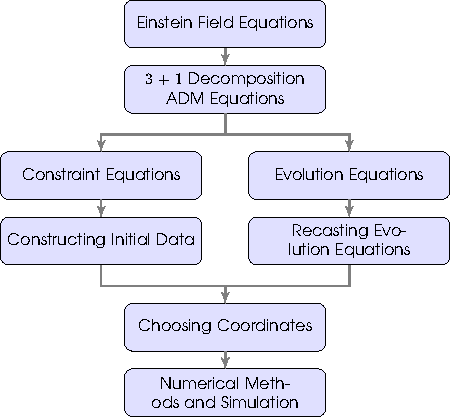
\includegraphics{figures/basic_idea_scheme.pdf}
    \end{frame}
  % section the_basic_idea (end)

  \section{The Details} % (fold)
  \label{sec:the_details}
    \subsection{$3+1$ Decomposition} % (fold)
    \label{sec:section_name}
      \begin{frame}{$3+1$ Decomposition: The ADM Equations}
        Constraint Equations:
        \begin{mybox}
          \begin{align*}
            R+K^2 - K_{ij}K^{ij} &= 16 πρ \\
            D_j\roundBrackets{K^{ij} - γ^{ij}K} &= 8 πS^i
          \end{align*}
        \end{mybox}
        \[
          ρ \define n_a n_b T^{ab}
          \separate
          S^i \define -γ^{ij}n^a T_{aj}
        \]
      \end{frame}

      \begin{frame}{$3+1$ Decomposition: The ADM Equations}
        Evolution Equations:
        \begin{mybox}
          \begin{align*}
            \partial_t γ_{ij} &= -2α K_{ij} + D_i β_j + D_jβ_i \\
            \partial_t K_{ij} &= α\roundBrackets{R_{ij} - 2K_{ik}K^k_j + KK_{ij}} - D_iD_jα - 8πα\boxBrackets{S_{ij} - \frac{1}{2}γ_{ij}\roundBrackets{S - ρ}} \\
            &+ β^kD_kK_{ij} + K_{ik} D_jβ^k + K_{kj} D_iβ^k
          \end{align*}
        \end{mybox}
        \[
          S_{ij} \define γ_{ia}γ_{jb}T^{ab}
          \separate
          S \define γ^{ij}S_{ij}
        \]
      \end{frame}
    % subsection section_name (end)

    \subsection{Constructing Initial Data} % (fold)
    \label{sec:constructing_initial_data}
      \begin{frame}{Constructing Initial Data: CTT Decomposition}

        Solve Constraint Equations for $W^i$ and $ψ$:
        \begin{mybox}
          \begin{align*}
            \roundBrackets{\bar{\laplacian}_L W}^i - \frac{2}{3} ψ^6 \bar{γ}^{ij} \bar{D}_j K &= 8π ψ^{10} S^i \\
            8\bar{D}^2 ψ - ψ\bar{R} - \frac{2}{3}ψ^5 K^2 + ψ^{-7} \bar{A}_{ij} \bar{A}^{ij} &= -16 π ψ^5 ρ
          \end{align*}
        \end{mybox}
        \[
          \bar{A}^{ij} = \bar{A}^{ij}_\mathrm{TT} + \roundBrackets{\bar{L}W}^{ij}
        \]
      \end{frame}

      \begin{frame}{Constructing Initial Data: CTT Decomposition}
        Construct Physical Solution:
        \begin{mybox}
          \begin{align*}
            γ_{ij} &= ψ^4 \bar{γ}_{ij} \\
            K_{ij}
              &= A_{ij} + \frac{1}{3}γ_{ij}K \\
              &= ψ^{-2} \bar{A}_{ij} + \frac{1}{3} γ_{ij} K
          \end{align*}
        \end{mybox}
      \end{frame}
    % subsection constructing_initial_data (end)

    \subsection{Choosing Coordinates} % (fold)
    \label{sec:choosing_coordinates}
      \begin{frame}{Choosing Coordinates: The Lapse and Shift}
        Geodesic Slicing:
        \begin{mybox}
          \[
            α = 1
            \separate
            β^i = 0
          \]
        \end{mybox}
        \bigskip

        \pause
        Maximal Slicing:
        \begin{mybox}
          \[
            D^2α = α \boxBrackets{K_{ij}K^{ij} + 4π \roundBrackets{ρ + S} }
          \]
        \end{mybox}
      \end{frame}
    % subsection choosing_coordinates (end)

    \subsection{Recasting The Evolution Equations} % (fold)
    \label{sec:recasting_the_evolution_equations}
      \begin{frame}{Recasting the Evolution Equations: The BSSN Formalism}
        Idea:
        \begin{mybox}
          \begin{align*}
            γ_{ij} &= e^{4φ} \bar{γ}_{ij} \\
            K_{ij} &= e^{4φ} \tilde{A}_{ij} + \frac{1}{3}γ_{ij}K
          \end{align*}
        \end{mybox}
      \end{frame}
    % subsection recasting_the_evolution_equations (end)

    \subsection{Numrical Methods} % (fold)
    \label{sec:numrical_methods}

    % subsection numrical_methods (end)
  % section the_details (end)


  \section{Results} % (fold)
  \label{sec:results}
    \begin{frame}
      Visualizing the results:
      \begin{itemize}
        \item{
          \href{run:videos/sxs-vortex-tendex_visualization-head-on_collision.mp4}{\beamergotobutton{SXS: BBH head-on collision}}
          \href{https://www.youtube.com/watch?v=4nM6kf2OAFw}{\beamergotobutton{Web Version}}
        }
        \item{
          \href{run:videos/sxs-demo_binary_orbit_and_collision.mp4}{\beamergotobutton{SXS: BBH orbit and collision}}
          \href{https://www.youtube.com/watch?v=p647WrQd684}{\beamergotobutton{Web Version}}
        }
        \item{
          \href{run:videos/sxs-highly-precessing_bbh_run.mp4}{\beamergotobutton{SXS: Highly precessing BBH}}
          \href{https://www.youtube.com/watch?v=grA5KfDlsAY}{\beamergotobutton{Web Version}}
        }
      \end{itemize}
      \bigskip

      Going Further:
      \begin{itemize}
        \item{
          \href{run:videos/nasa-colliding_neutron_stars_create_black_hole_and_gamma-ray_burst.webm}{\beamergotobutton{NASA: Colliding Neutron Stars}}
          \href{https://www.youtube.com/watch?v=ow9JCXy1QdY&t=2s}{\beamergotobutton{Web Version}}
        }
      \end{itemize}
    \end{frame}
  % section results (end)

  \begin{frame}
    \frametitle{References}
    \scriptsize
    \begin{multicols}{2}
      \nocite{*}
      \bibliography{references}
    \end{multicols}
  \end{frame}

\end{document}